\chapter{Literature Review}
\phantomsection
\label{ch:literature}

\section{Overview}
\phantomsection
\label{sec:ocr-overview}
This chapter provides a comprehensive literature review covering several 
key aspects of Optical Character Recognition (OCR). 
It begins with a definition of OCR, followed by an overview of its technological
 evolution over time. Particular attention is given to the unique challenges 
 associated with Khmer OCR, a low-resource language with complex script characteristics.
  The chapter also explores the significant role of synthetic data in addressing data 
  scarcity for low-resource language processing and dataset development.
   Finally, the chapter concludes by identifying and summarizing the existing 
   research gaps in the current literature, highlighting areas that remain 
   under-explored and underscoring the need for further investigation.


\section{Definition of Optical Character Recognition (OCR)}
\phantomsection
\label{sec:ocr-definition}
Optical Character Recognition (OCR) is a field of computer vision and pattern recognition
 that focuses on the automatic identification and digitization of printed or handwritten 
 text from images, scanned documents, or other visual media \cite{singh2012survey}. 
 OCR systems aim to convert visual representations of text into machine-encoded formats, 
 enabling automated indexing, editing, and data extraction \cite{muaz2015khmerocr}.

Modern OCR technology has evolved significantly from its early rule-based and template-matching
roots to incorporate advanced machine learning techniques, particularly deep learning,
which allow for improved accuracy in character detection, segmentation, and classification across 
diverse languages and scripts.

OCR systems typically consist of several key components: image preprocessing (e.g., noise removal, binarization), text detection, character segmentation, feature extraction, and recognition. These systems must be adapted to handle various font styles, image distortions, complex layouts, and script-specific features. While OCR for Latin-based languages has become highly accurate, extending such systems to non-Latin scripts—such as Khmer—remains a significant research challenge due to unique linguistic and structural characteristics.
   
\section{Evolution of OCR Technology}
\phantomsection
\label{sec:synthetic-data}
Nowadays, optical character recognition (OCR), plays an instrumental role in extracting text from images,
scanned documents, and other visual media. pattern recognition technology took shape almost 100 years ago.
Many iterations later, it evolved into optical character recognition (OCR) systems solutions that are
now being used.

Fast-forwarding to the present, this technology is used by organizations to digitize their documents, because
of they want to convert unstructured data into structured data such as document, PDFs, and images into
machine-readable text.

In this section, we cover the history of OCR technology: how it began, 
how it has changed through time, and its current state.

\subsection{Early Concepts (1920s-1930s)}
\phantomsection
OCR technology has ties to telegraphy. Around the time of the First World War, 
typewriters and telegraphs were already in use. Physicist Emanuel Goldberg invented a
machine that could read characters and convert them into telegraph code. 

In the 1920s, he went further and created the first electronic document retrieval system. 
While businesses were microfilming financial records at that time, retrieving specific 
records from films was still impossible. To overcome this shortcoming, Goldberg used a 
photoelectric cell for pattern recognition using a movie projector, and this machine was 
called “The Statistical Machine.”  

The machine could sort mail and decipher bank checks through patterns that were unseen by the human eye. 

\begin{figure}[ht]
    \centering
    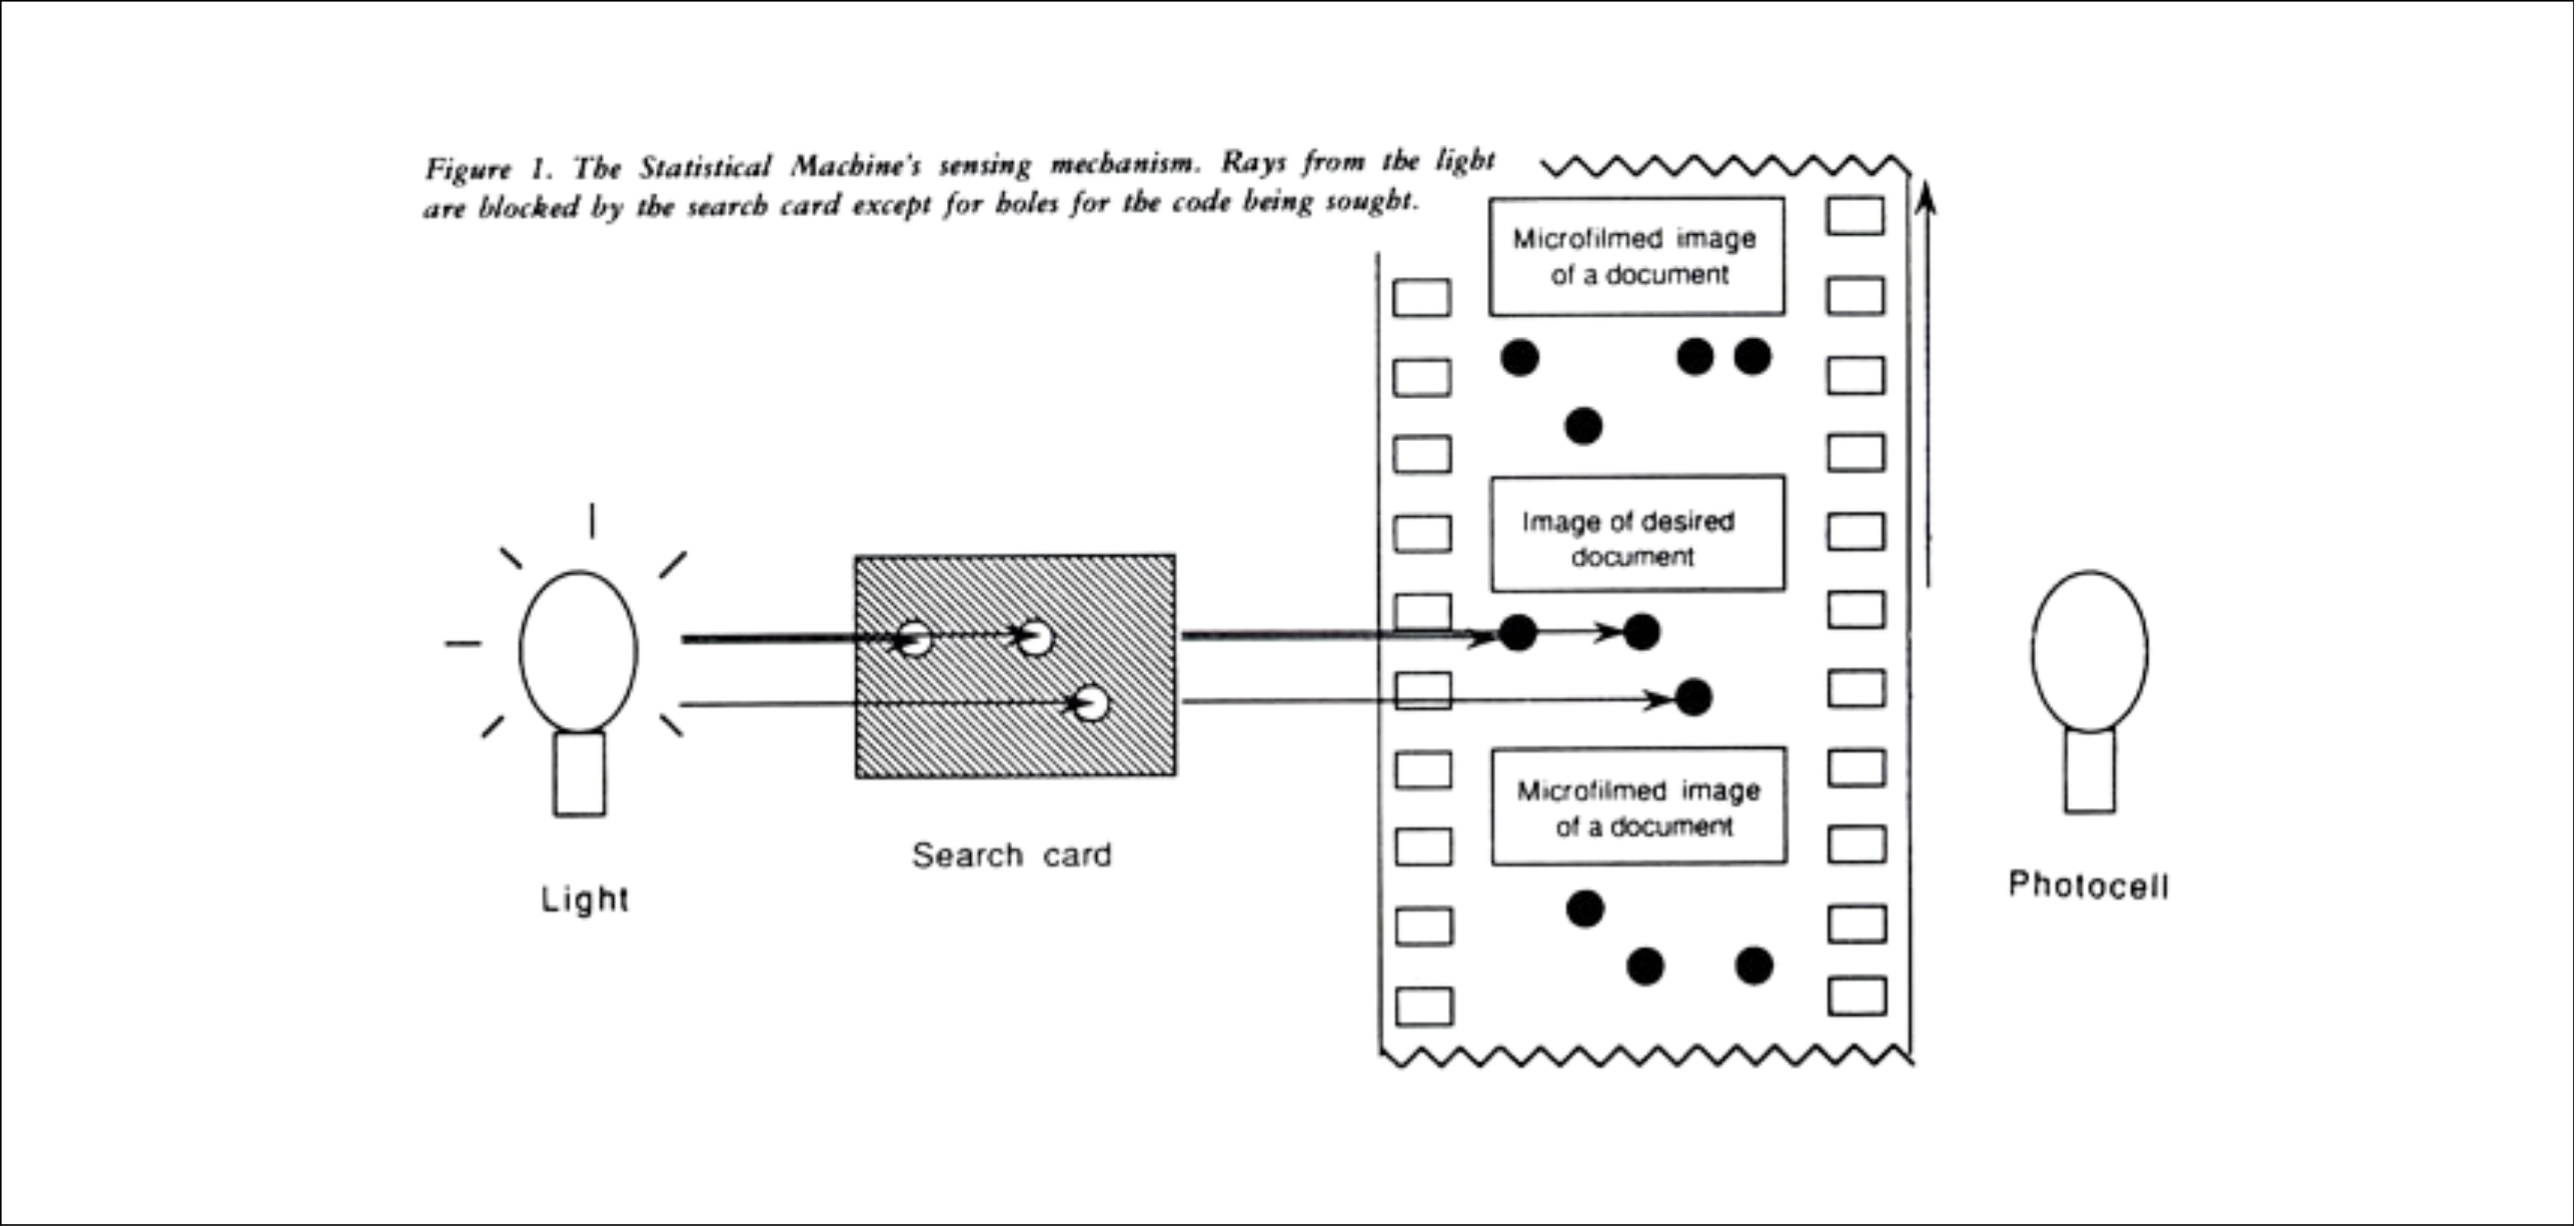
\includegraphics[width=1\textwidth]{figures/statistical_machine_diagram.png}
    \caption{Diagram of Emanuel Goldberg's Statistical Machine (1920s)}
    \label{fig:statistical-machine}
\end{figure}

\subsection{Analog Reading Machine (1930s)}
\phantomsection
\label{sec:analog-reading}

In 1929, Gustav Tauschek, a self-taught Austrian inventor, built upon Goldberg's pioneering work
by adapting the photoelectric detector concept to create his innovative Analog Reading Machine. 
This mechanical marvel represented a significant advancement in early optical character recognition
technology, demonstrating the potential for automated text recognition systems \cite{diem2010recognizing}.

The Reading Machine featured a sophisticated scanning mechanism with a small viewing window designed
to capture text images. As documents passed through this window, an ingeniously designed 
rotating disk system would engage. This disk, meticulously crafted with precise cutouts 
representing various numbers and alphabetic characters, served as the machine's template matching system,
a concept that would later influence modern pattern recognition approaches \cite{diem2010recognizing}.

The operation was remarkably elegant: when the scanned text matched one of the disk's cutout patterns, 
the machine would automatically activate its printing mechanism. A synchronized printing drum would 
then imprint the corresponding characters onto paper, effectively translating visual text into printed 
output. This mechanical automation represented one of the earliest examples of automated text 
recognition and reproduction, laying important groundwork for future OCR developments.

While limited by today's standards, Tauschek's invention demonstrated remarkable ingenuity 
in mechanical pattern recognition and automated text processing. The machine could process 
approximately 80 characters per minute, a significant achievement for its time, though it was 
primarily limited to recognizing printed text in specific fonts and formats, highlighting the 
challenges of character recognition that persist in modern OCR systems \cite{diem2010recognizing}.

\begin{figure}[ht]
    \centering
    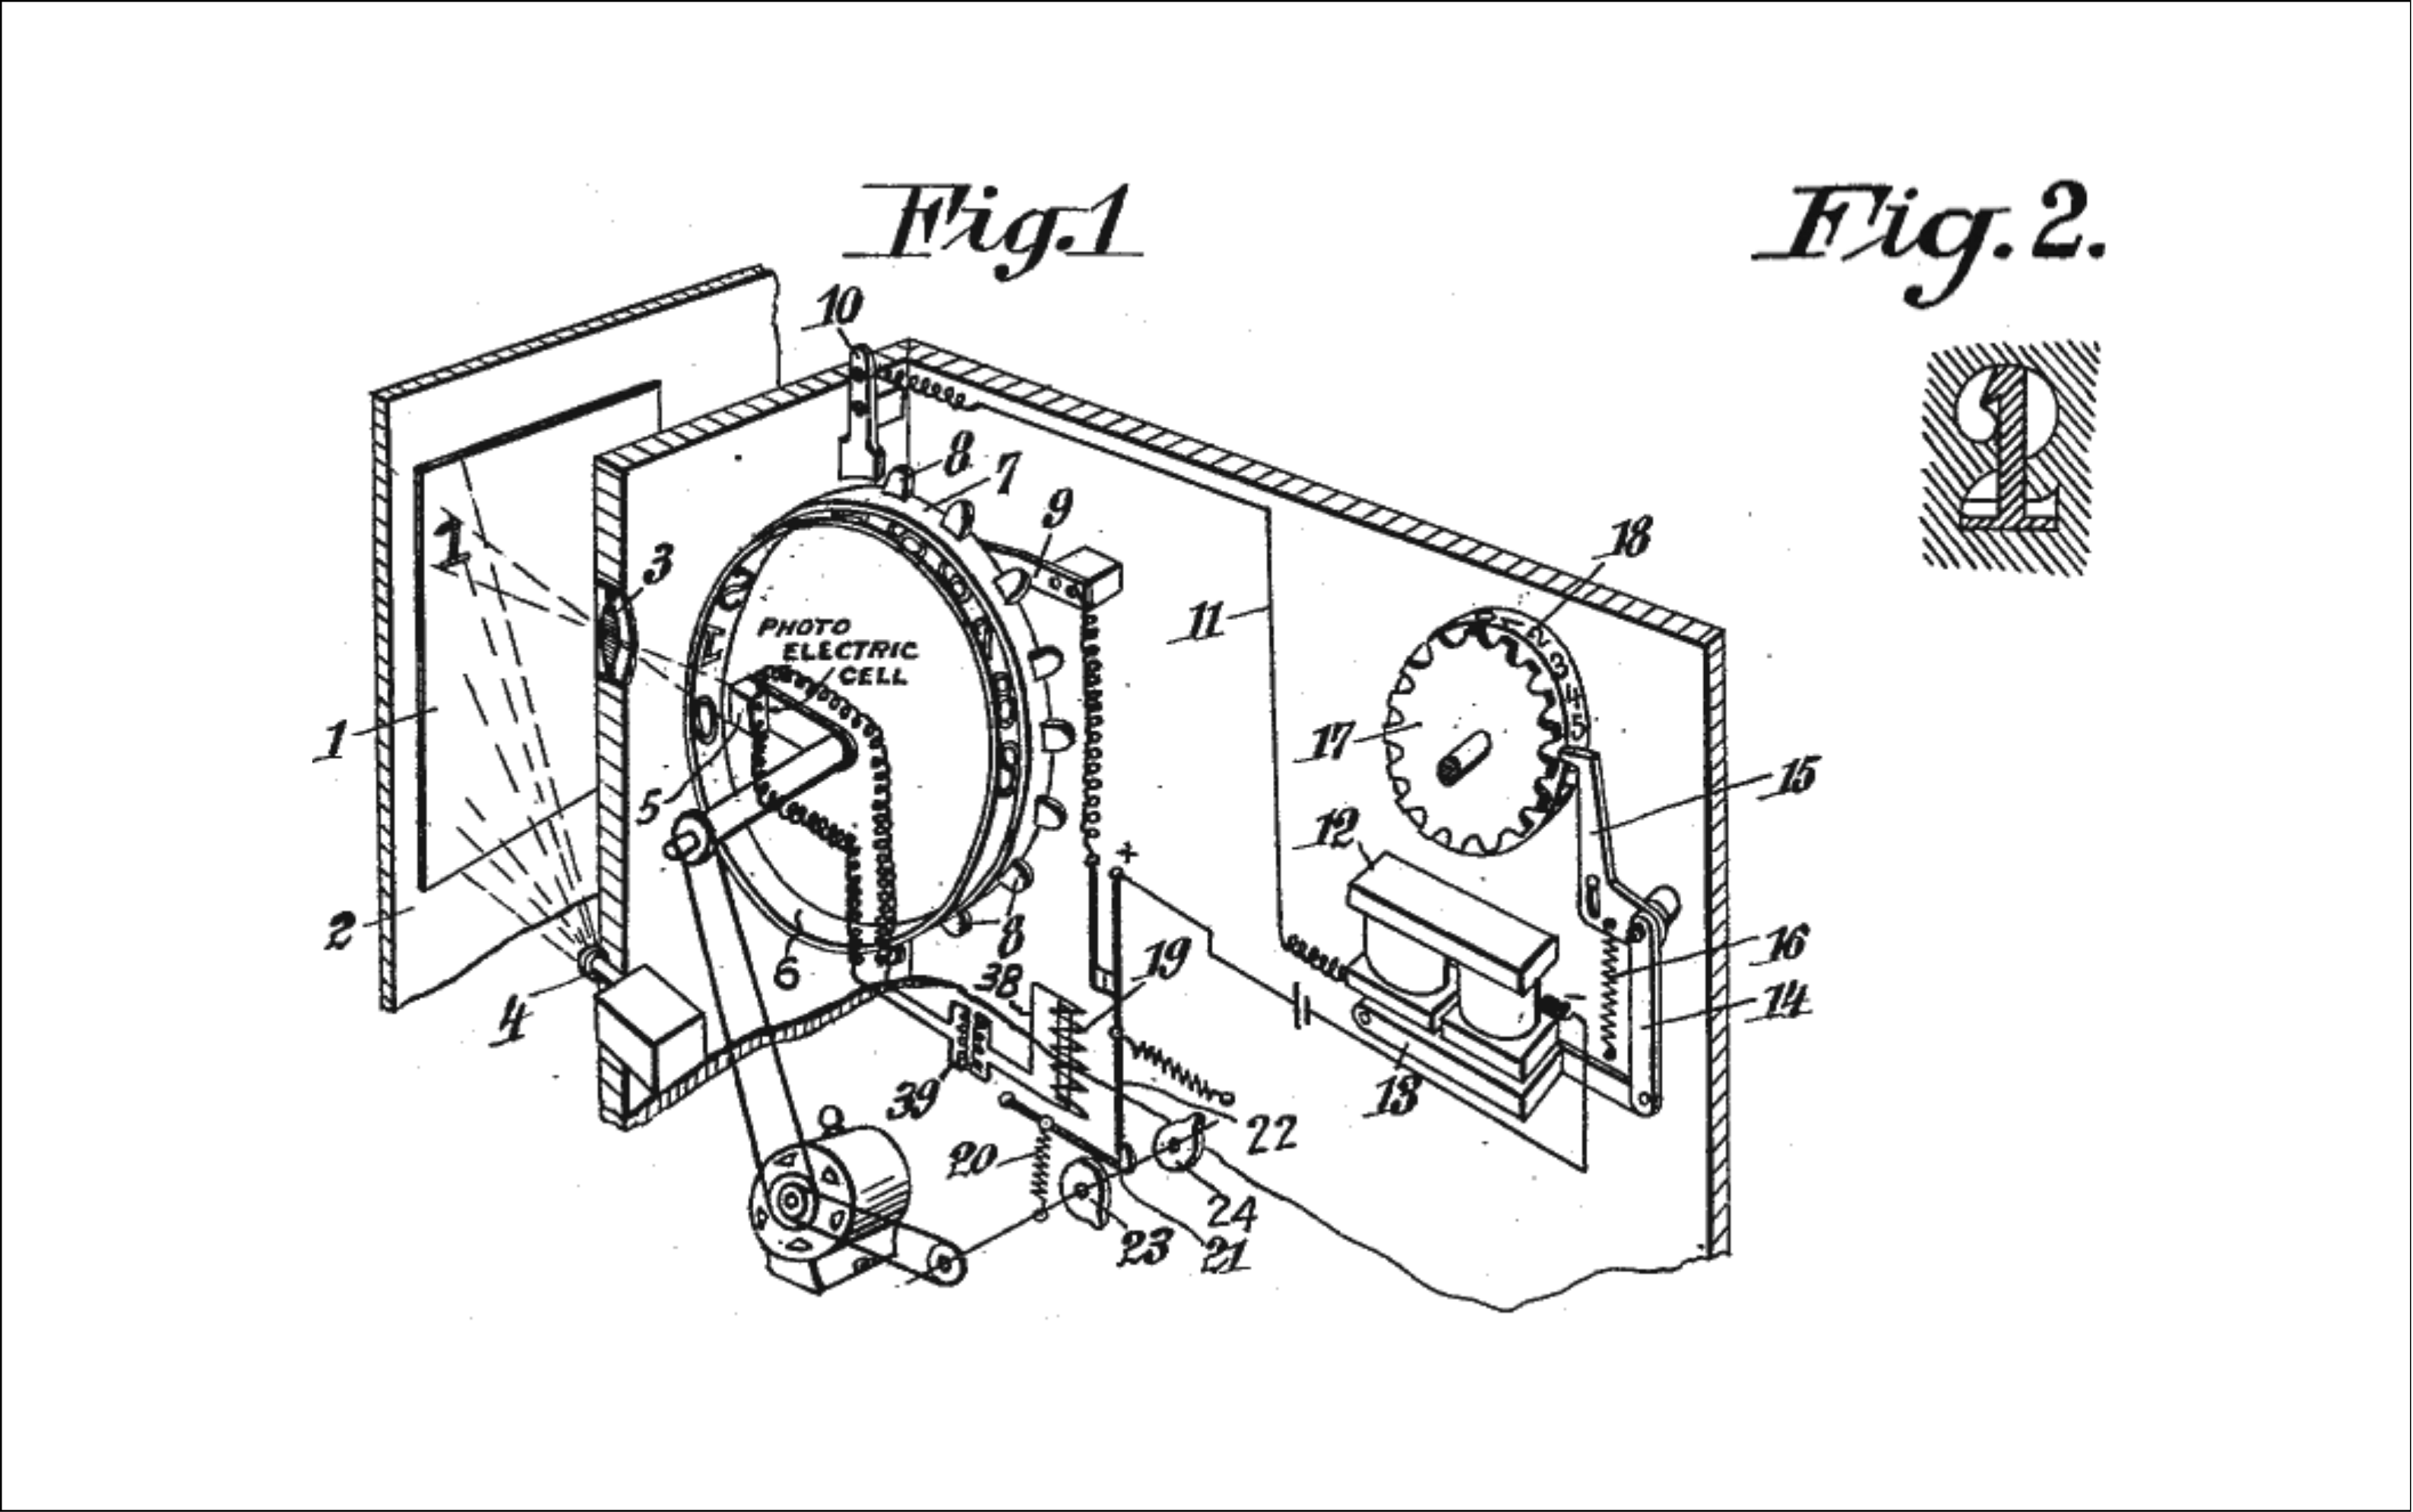
\includegraphics[width=1\textwidth]{figures/Analog_Reading_Machine.png}
    \caption{Tauschek's Analog Reading Machine (1930s) \cite{diem2010recognizing}}
    \label{fig:analog-reading}
\end{figure}


\subsection{First OCR Machine (1950s)}
\phantomsection
\label{sec:first-ocr}

The 1950s were a transformative decade in the history of technology. 
As industries began to generate and rely on increasingly large volumes of data, 
the demand for efficient and automated data processing systems grew significantly. 
Traditional reading machines at the time were limited—they could scan physical 
documents but lacked the ability to translate printed text into digital, machine-readable 
formats. This limitation posed a major challenge to organizations seeking to automate 
information management.

To address this issue, several innovators contributed groundbreaking ideas. Among them 
were David H. Shepard and Harvey Cook Jr., who developed one of the earliest optical character 
recognition (OCR) machines. Their invention, \cite{shepard1953gismo} known as GISMO, was a pioneering solution 
designed to interpret printed characters and convert them into computer-readable code. 
During the patent application process, it was referred to as the "Analyzing Reader."

GISMO represented a significant leap forward in automated data capture. Unlike earlier systems, 
it was capable of recognizing text visually and encoding it into a digital format—a 
foundational step toward the OCR systems we use today. This innovation played a crucial 
role in launching the field of document digitization and information automation, paving 
the way for modern advancements in machine reading and artificial intelligence.

\begin{figure}[ht]
    \centering
    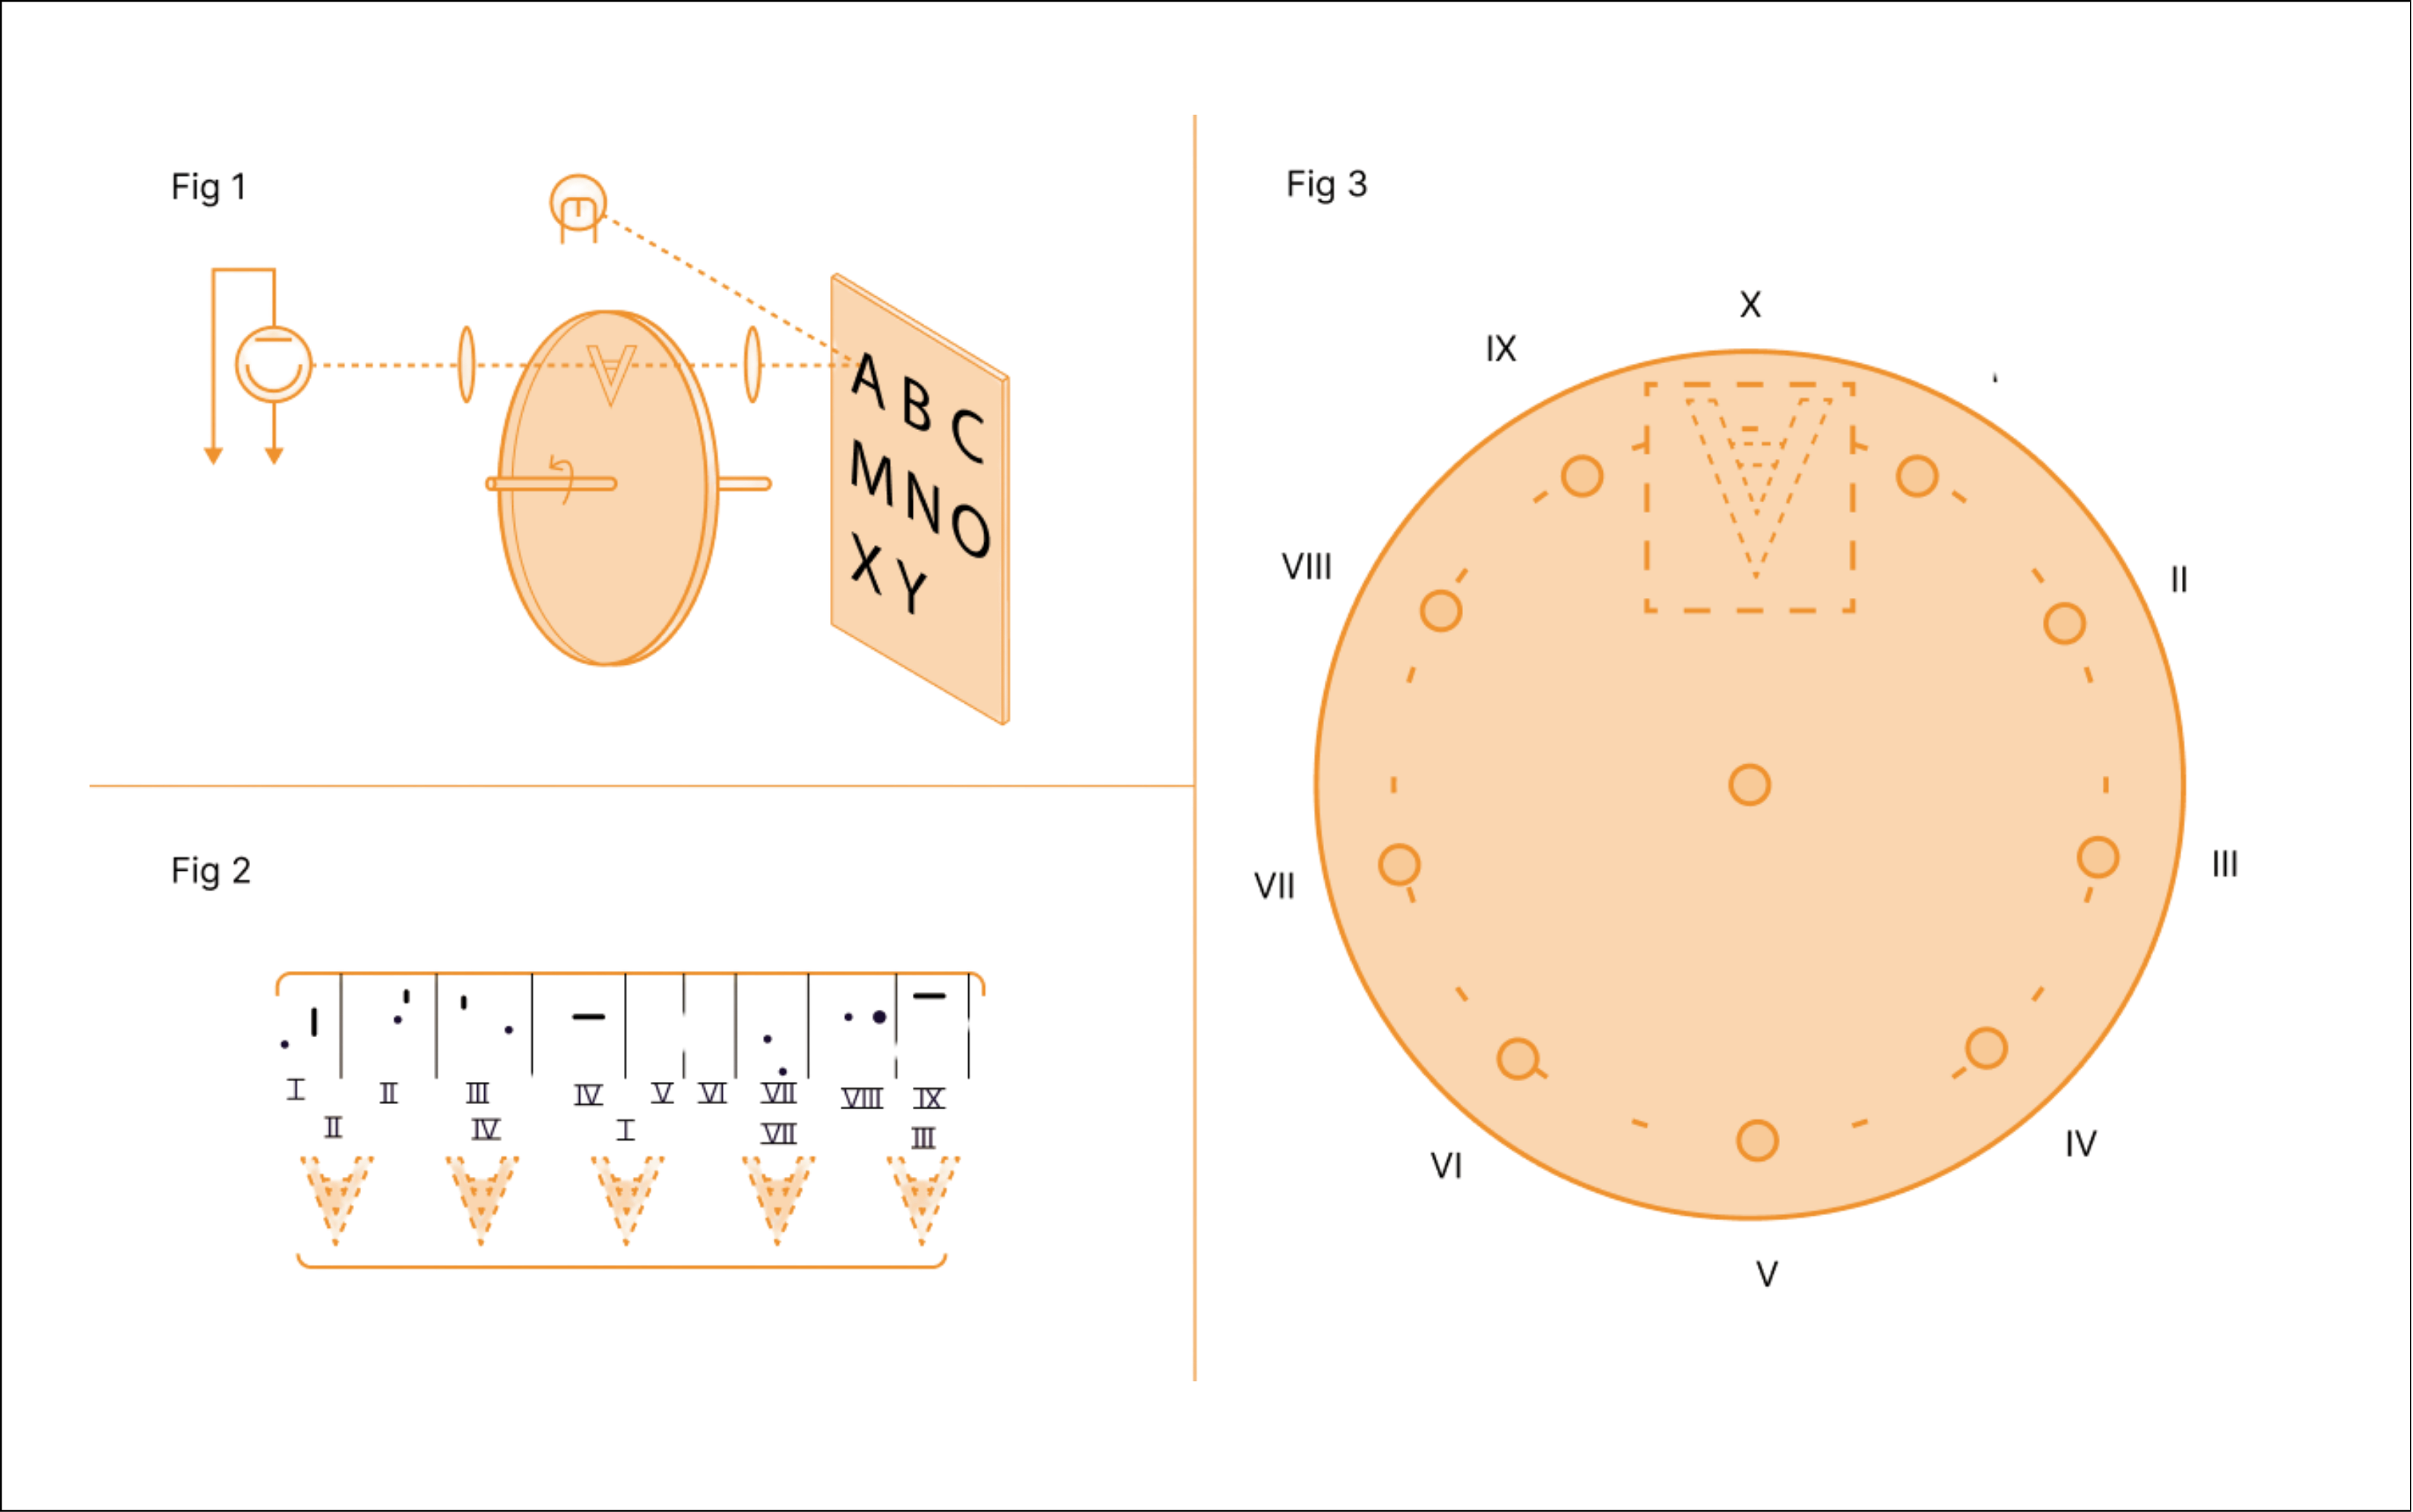
\includegraphics[width=1\textwidth]{figures/David_Shepard_ocr.png}
    \caption{David Shepard's GISMO - The First OCR Machine (1950s) \cite{docsumo2023ocr}}
    \label{fig:shepard-ocr}
\end{figure}

\subsection{Pattern Recognition Advancements (1960s-1970s)}
\phantomsection
\label{sec:pattern-recognition}

In the 1960s, researchers at the Massachusetts Institute of Technology (MIT)  
began working on ways to improve early Optical Character Recognition (OCR) systems. 
Their main goal was to create software that could adapt to different types of documents, 
such as those with various layouts, fonts, and print qualities. They wanted the OCR systems 
to be more flexible and intelligent in how they interpreted scanned text. However, 
the technology at that time had serious limitations. The computers were slow and had 
very little memory, making it difficult to run advanced algorithms. As a result, although 
the researchers had innovative ideas, they couldn't fully implement or test them. These 
efforts, however, laid the foundation for what would later become machine learning in 
OCR — where systems can actually learn and improve over time by processing large amounts of data.

Around the same time, researchers Richard Duda and Peter Hart introduced a powerful new method 
called the Hough Transform \cite{duda1972use}. This algorithm was designed to detect simple 
geometric shapes, such as lines and circles, within images. In the context of OCR, 
this meant machines could now identify the structure of documents — for example, 
where lines of text began and ended, or where printed shapes like logos or seals were located. 
This was a big step forward because it helped OCR systems better understand how to separate 
and process the contents of a page.


Despite its strengths, the Hough Transform also had its downsides. It required a lot of 
computing power and could be sensitive to image noise or low-quality scans. In addition, 
it was designed mainly for detecting basic shapes, not for understanding or recognizing 
complex characters or handwritten text.

In comparison to modern OCR technology, today’s systems use deep learning models like 
convolutional neural networks (CNNs) and transformers (e.g., TrOCR), which can automatically 
detect and recognize characters without needing explicit shape-detection steps. These modern 
systems are much faster, more accurate, and can handle noisy or complex documents far better 
than the early methods like the Hough Transform. Still, the foundational ideas from the 
1960s — including adaptive algorithms and shape detection — played an important role in 
getting us to where we are now. 

\begin{figure}[ht]
    \centering
    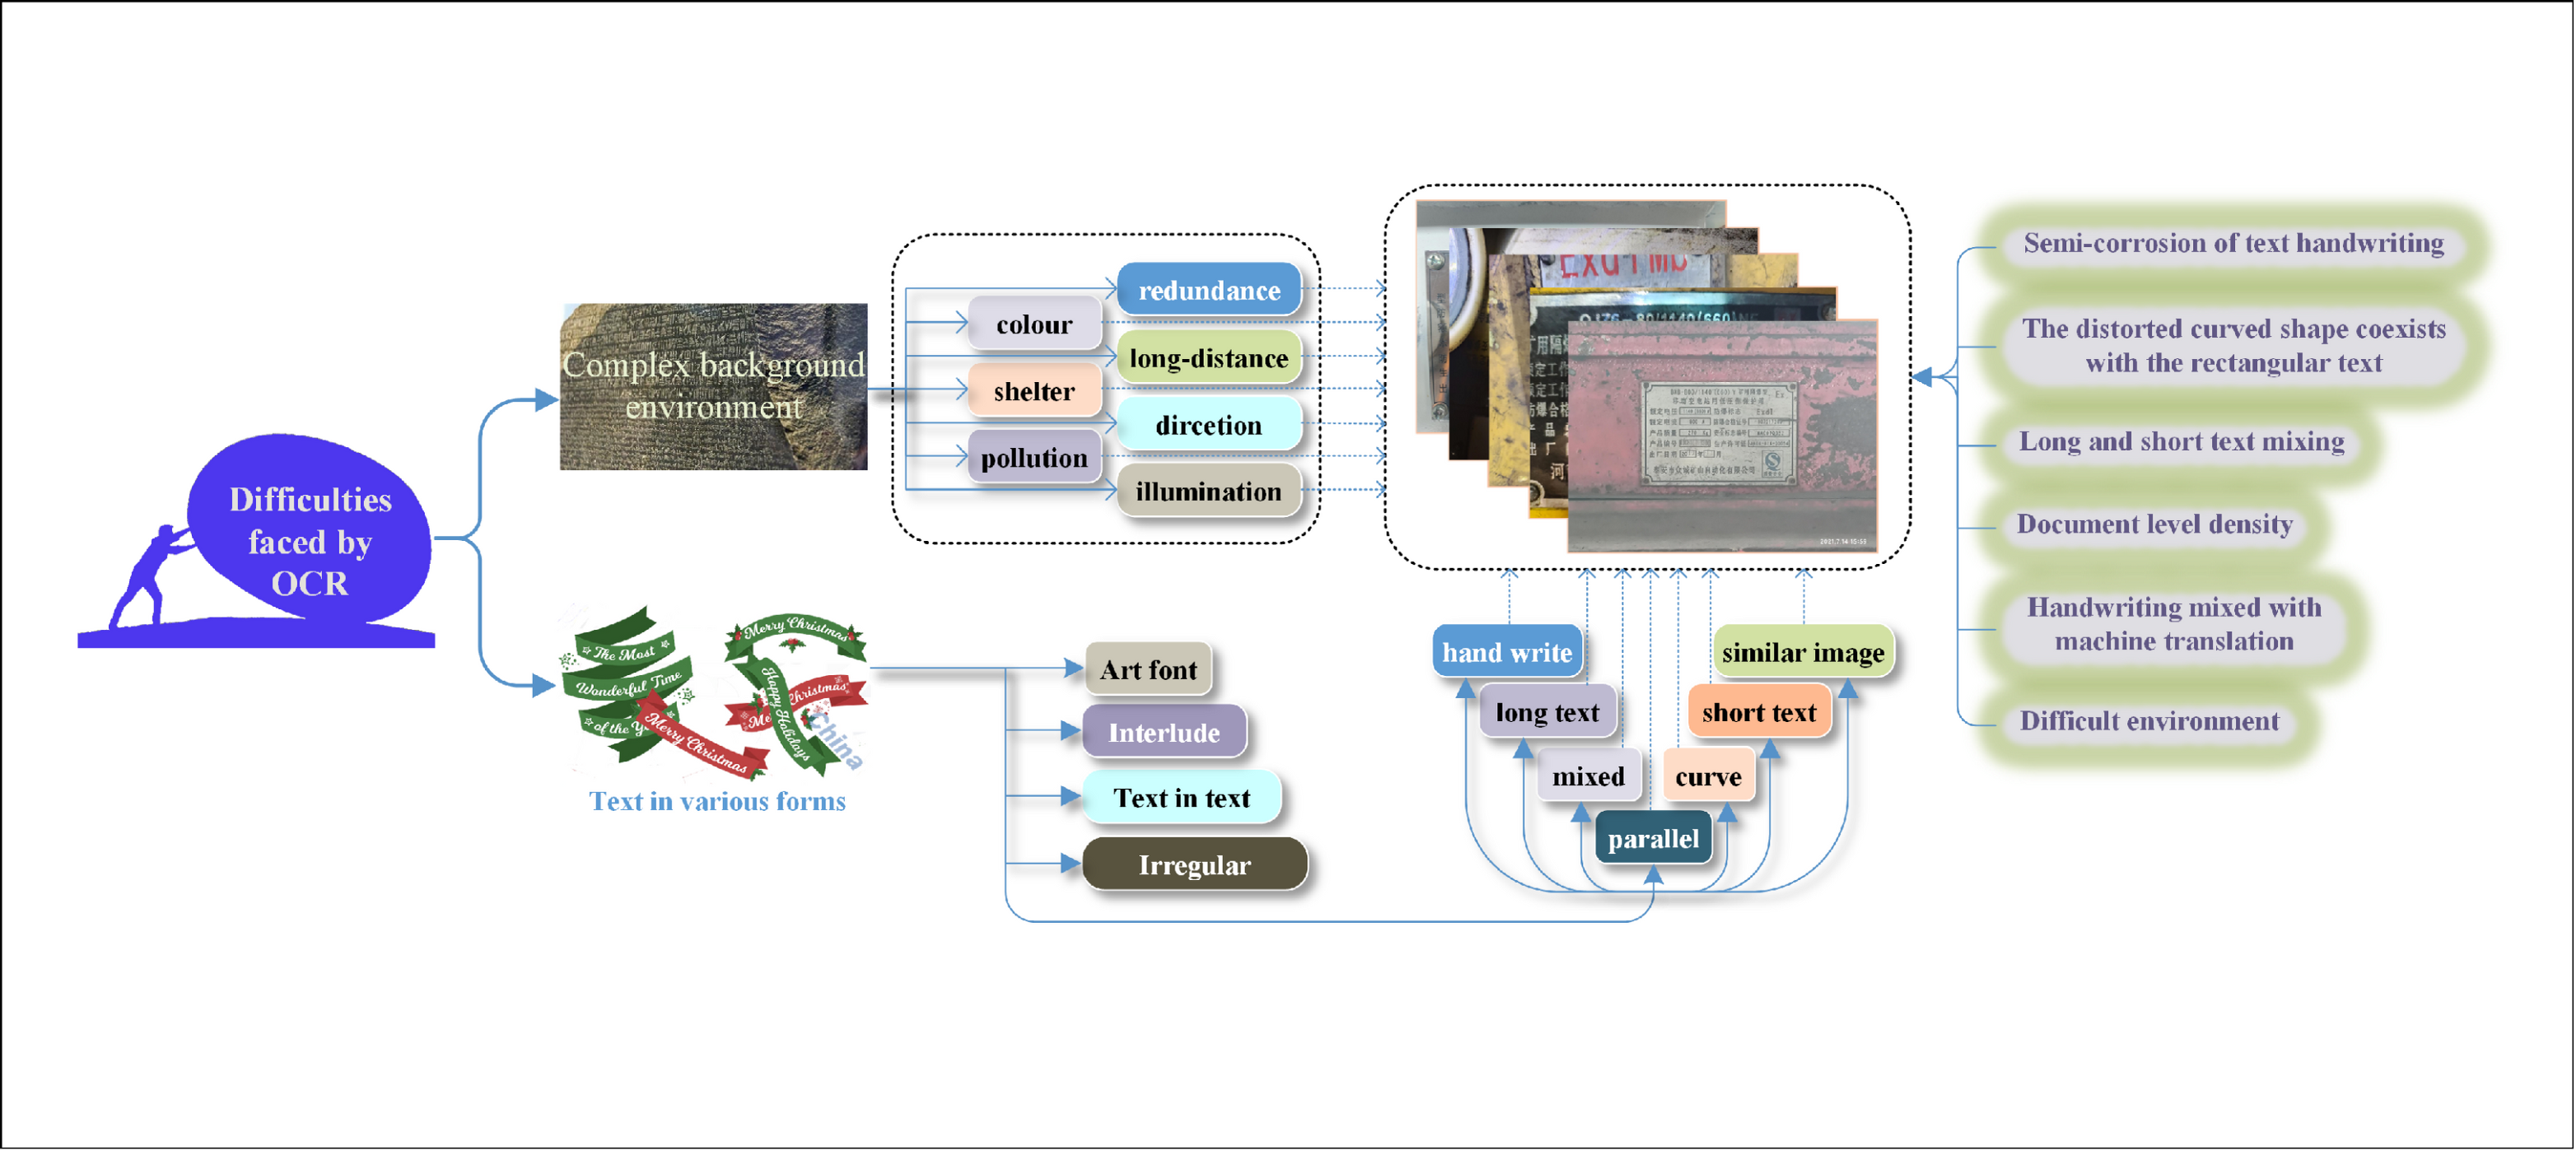
\includegraphics[width=1\textwidth]{figures/Hough_Transform_technique.png}
    \caption{Illustration of the Hough Transform technique developed in the 1960s, 
    which enabled OCR systems to detect geometric features such as lines and circles 
    within scanned documents. This method enhanced document layout analysis and text 
    line segmentation, forming a foundational step in the evolution of 
    structure-aware text detection \cite{liu2023hough}.}
    \label{fig:hough-transform}
\end{figure}

\subsection{ICR and MICR (1960s-1970s)}
\phantomsection
\label{sec:icr-micr}

Amid the evolving landscape of OCR technology in the 1960s and 1970s, two notable 
technologies emerged - Intelligent Character Recognition (ICR) and Magnetic Ink Character 
Recognition (MICR) \cite{phyu2009hybrid}.

\subsubsection{2.3.5.1 Intelligent Character Recognition (ICR)}
\phantomsection
\label{sec:icr}

As the demand for handwritten text recognition grew, researchers came up with the ICR technology. 
MIT's pioneering research group refined OCR's capabilities to decipher handwritten characters, 
marking the birth of the ICR algorithm. This laid the foundation for future machine learning-driven 
advancements, set to revolutionize OCR technology.

\subsubsection{2.3.5.2 Magnetic Ink Character Recognition (MICR)}
\phantomsection
\label{sec:micr}

In the banking industry, the need for efficient check processing led to the development 
of MICR technology. By embedding magnetic ink characters in checks, automated systems can 
rapidly read and process these documents. This innovation streamlined financial operations 
and illustrated OCR's practical applications beyond traditional text.




\subsection{Tesseract OCR (2005-2021)}
\phantomsection
\label{sec:tesseract-ocr}
In the early 2000s, there weren’t many major improvements in OCR technology, 
either in hardware or software. However, things changed in 2005 when the Tesseract OCR 
engine was brought back as an open-source project. This gave new life to OCR development.

Tesseract was first created by Hewlett-Packard in the 1980s, but it wasn’t widely 
used until it was released to the public by Google as open-source software. 
This meant that anyone could download it, use it for free, and even improve it.

The updated version of Tesseract included modern machine learning and computer vision 
techniques. It was able to recognize and extract text from images with much better 
accuracy than before. Developers could use Tesseract  \cite{smith2007overview} directly or through an API 
(Application Programming Interface), which made it easier to include OCR features 
in other apps and systems. Thanks to this release, Tesseract became one of the 
most popular and reliable OCR tools in the world.

\begin{figure}[ht]
    \centering
    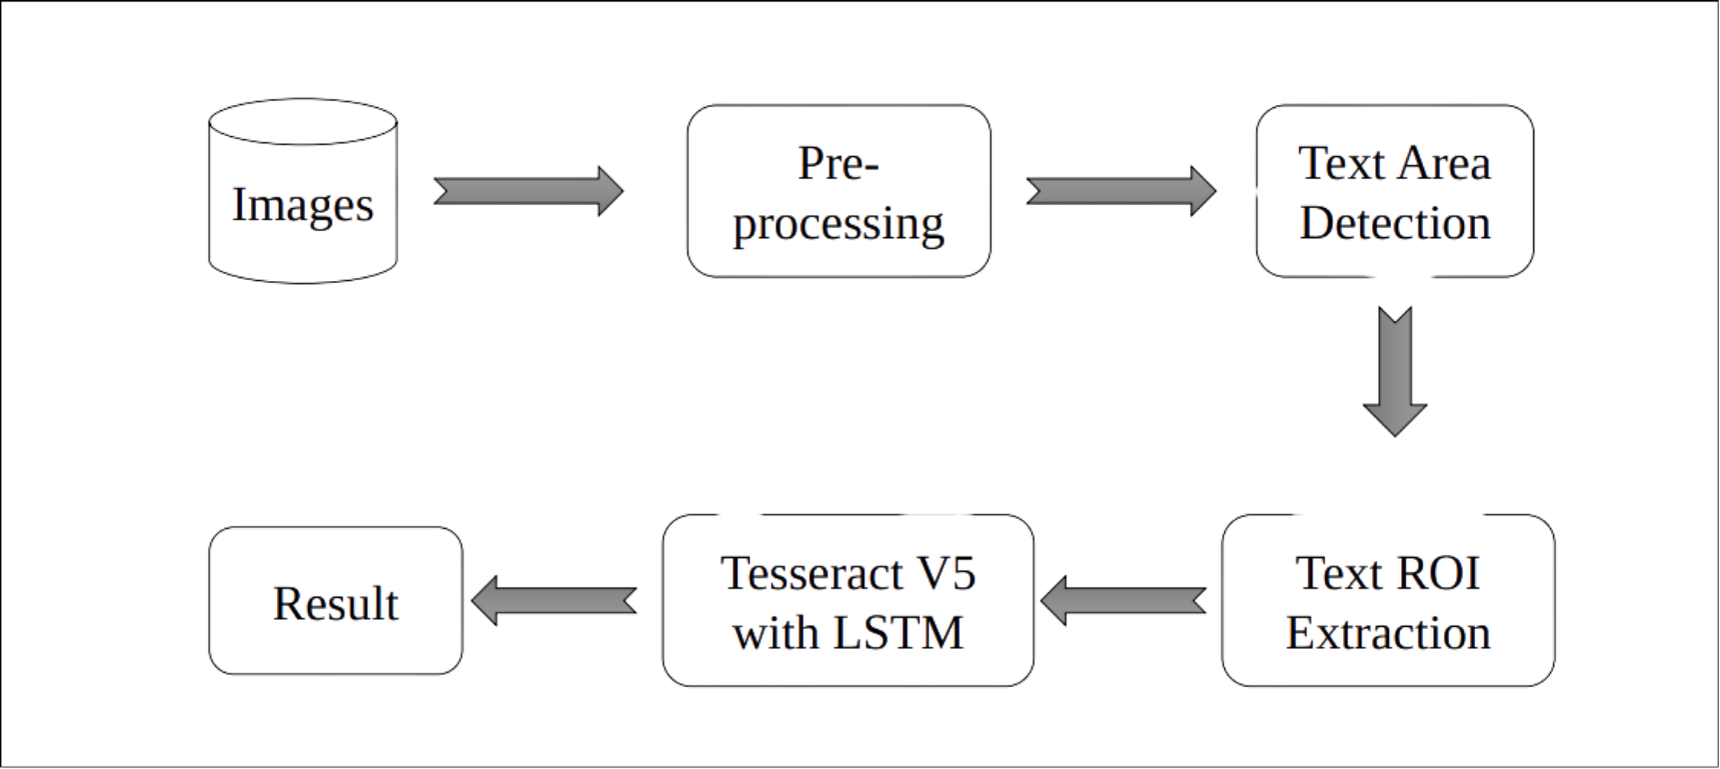
\includegraphics[width=\textwidth]{figures/Tesseract.png}
    \caption{Illustration of Tesseract OCR engine advancements, showing the improvement 
    of recognition accuracy over time and its ability to extract text from complex images \cite{
    zacharias2020tesseract}}
    \label{fig:tesseract_advancements}
\end{figure}

\subsection{Advancements in Khmer OCR (2021-Present)}
\phantomsection
\label{sec:advancements-in-khmer-ocr}

The new Khmer OCR system is built using a sequence-to-sequence (Seq2Seq) 
deep learning model with attention. Instead of recognizing each character separately, 
the model looks at a whole line of text and understands it as a sequence, 
just like how we read. It starts with an encoder that uses convolutional layers 
to extract visual features from the image and then passes these features 
through a Gated Recurrent Unit (GRU), which captures the order of the characters.

The decoder then takes this information and generates the output text, one character 
at a time. With the help of an attention mechanism, the decoder can focus on different 
parts of the image while predicting each character. This allows the model to handle 
long text lines and various font styles more effectively.

The model was trained on thousands of computer-generated Khmer text images using seven 
common fonts. On a test set of 3,000 images, it achieved a character error rate (CER) 
of only 1\% \cite{buoy2021seq2seq}, which is significantly better than the 3\% \cite{buoy2021seq2seq} CER from Tesseract OCR for Khmer. 
This shows the model's high accuracy and reliability.

Compared to older OCR tools like Tesseract, which treat text as a series of separate 
characters, this new end-to-end model sees the text as a whole sequence. 
This helps it better understand context and spacing. It also adapts better 
to different fonts and styles, especially in complex scripts like Khmer. 
The attention mechanism is a major improvement because it lets the model decide 
where to "look" in the image while decoding, which improves accuracy in challenging cases.

In short, this Khmer OCR model uses modern AI to provide faster, smarter, and 
more accurate text recognition, especially for a language that has been 
underserved in OCR research.

\begin{figure}[ht]
    \centering
    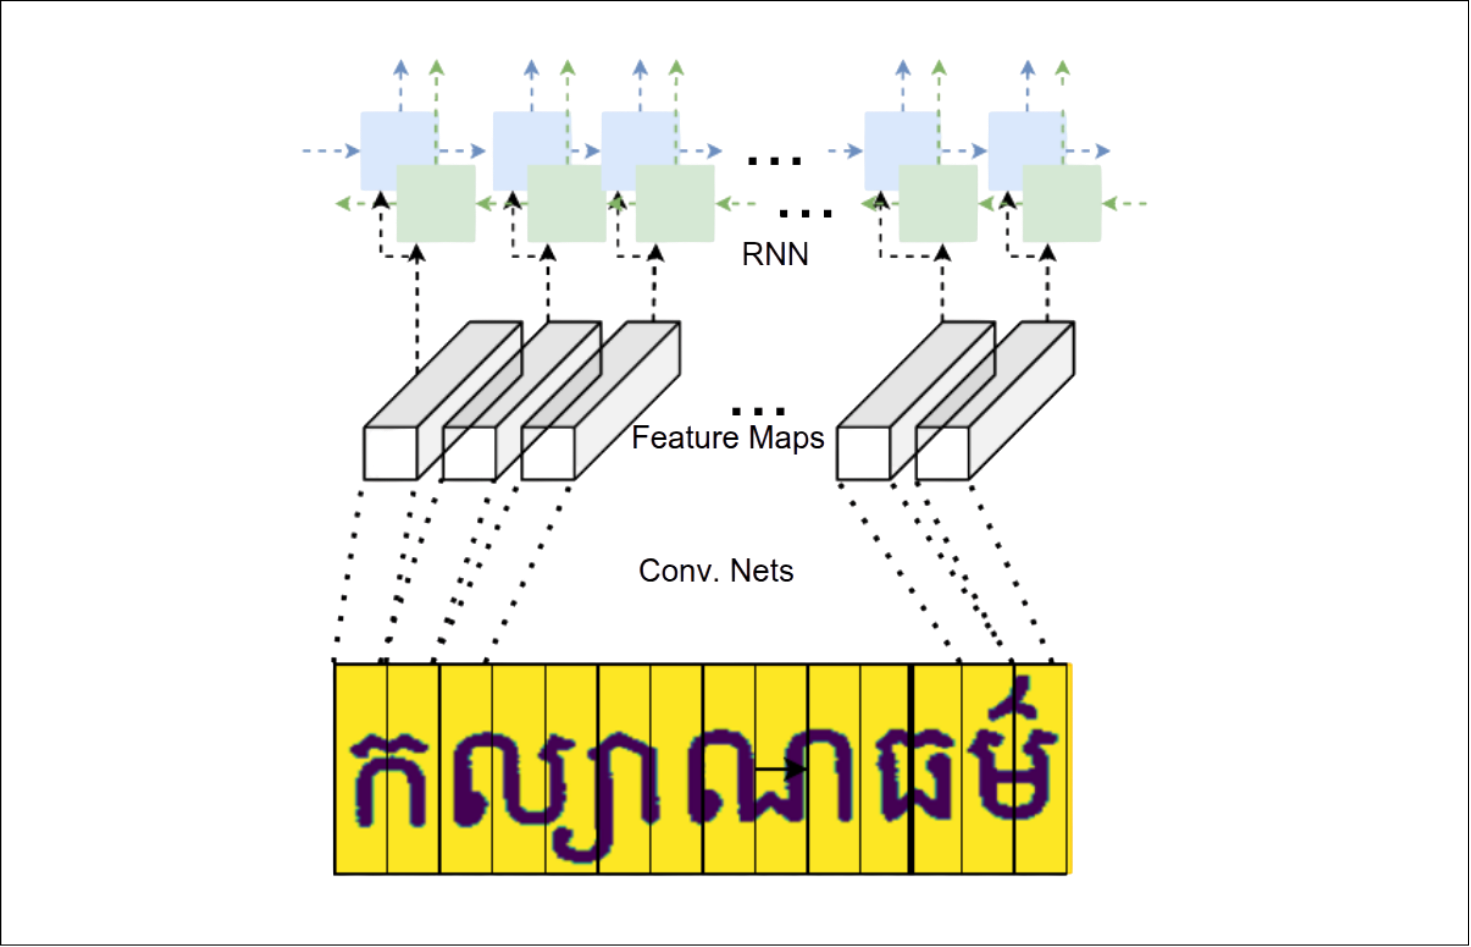
\includegraphics[width=\textwidth]{figures/bouy_rina_end_to_end_khmer_ocr.png}
    \caption{Illustration of the end-to-end Khmer OCR system proposed by Bouy and Rina,
    which combines a feature extractor, a sequence-to-sequence model,
     and a post-processing module to achieve high accuracy in recognizing Khmer text. \cite{buoy2021seq2seq}}
    \label{fig:bouy-rina-end-to-end-khmer-ocr}
\end{figure}


\section{Challenges in Khmer OCR}
\phantomsection
\label{sec:datasets}

One of the biggest challenges in Khmer OCR lies in the complexity of the Khmer script. 
Unlike Latin-based languages,  Khmer characters can be stacked and combined using 
subscript consonants (Coeng), \cite{buoy2021seq2seq} diacritics, and various vowel positions. These components 
can appear above, below, to the left or right, or even surround the base character. 
This spatial variability significantly complicates the segmentation and recognition 
process, especially for systems that rely on isolated character analysis.

Khmer script is written in a wide range of fonts, each with its own style and visual 
characteristics. \cite{buoy2021seq2seq} These differences affect how characters are formed and connected, 
making it difficult for OCR models to generalize well across different typefaces. 
An effective OCR system must therefore be font-invariant and capable of accurately 
recognizing characters in any common or uncommon font.

Khmer is considered a low-resource language in the fields of natural language 
processing and OCR. This means there are limited publicly available datasets, 
pretrained models, and tools. As a result, researchers face difficulty in 
training robust models without generating synthetic data or heavily augmenting 
existing datasets.

Older Khmer OCR systems typically rely on explicit character segmentation, 
breaking down the text into individual symbols before recognition. 
This approach is prone to failure when applied to real-world images that 
contain noise, uneven spacing, or distorted characters. \cite{buoy2021seq2seq} Since Khmer characters 
often overlap or combine, segmentation errors are common and negatively affect 
recognition accuracy.

\begin{figure}[ht]
    \centering
    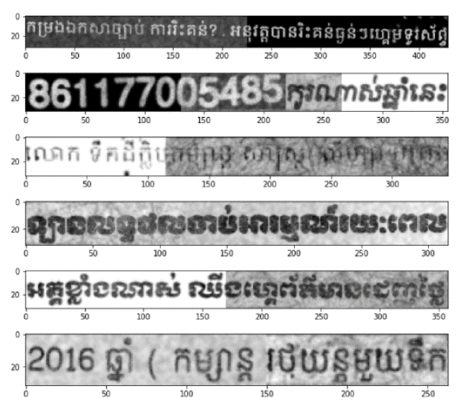
\includegraphics[width=\textwidth]{figures/overlap_segmentation.png}
    \caption{Khmer characters can overlap or combine in special ways, 
    making explicit segmentation prone to errors. \cite{buoy2021seq2seq}}
    \label{fig:overlap-segmentation}
\end{figure}

Prior Khmer OCR efforts have primarily focused on isolated character recognition 
and manual pre/post-processing steps. These systems are limited in their ability to 
recognize full words, phrases, or sentences. In contrast, an end-to-end solution can 
read an entire line of text and generate output in a single forward pass, 
improving speed, simplicity, and accuracy. \cite{buoy2021seq2seq}



\section{Role of Synthetic Data}
\phantomsection
\label{sec:dl-models}

To overcome the limitations of Khmer being a low-resource language, 
the authors created a large-scale synthetic dataset of Khmer \textbf{text-line} 
images using the open-source \textbf{text2image} tool provided by the Tesseract OCR engine.

The dataset was generated from a text corpus containing numbers, words, phrases, 
and full sentences in Khmer. \cite{buoy2021seq2seq} This corpus provided diverse linguistic content 
for rendering text-line images.

Multiple common Khmer fonts were used to render each item from the corpus. 
The variation in fonts helped train the model to be font-invariant and improve 
generalization across different writing styles.

The \textbf{text2image} tool was used to convert each text entry from the corpus into a 
grayscale image. The width and height of each image varied based on the text 
length and presence of stacked or subscript characters. All images were 
resized to a common height of 32 pixels to match the input size required 
by the neural network.

To simulate real-world challenges and improve the model's robustness, 
extensive data augmentation was applied \cite{buoy2021seq2seq} :
    \begin{itemize}
        \item Gaussian blurring
        \item Dilation and erosion
        \item Blob noise and speckle noise
        \item Multi-scale noisy backgrounds
        \item Random concatenation of augmented images
        \item Rotational and geometric distortions
    \end{itemize}

Each augmentation had a 50\% \cite{buoy2021seq2seq} chance of being applied to a given image, and multiple augmentations could be combined on a single image. This ensured that the model was trained on a wide range of noisy and distorted text scenarios.

The final synthetic dataset consisted of millions of images representing words, 
phrases, and sentences across different fonts and styles.

\section{Summary of Research Gaps}
\phantomsection
\label{sec:research-gaps}

This section identifies the key research gaps in the current literature on 
Khmer OCR technology. Despite advancements, several areas remain under-explored:

\begin{itemize}
    \item \textbf{Data Scarcity:} There is a lack of large-scale annotated datasets for Khmer text, which limits the training and evaluation of OCR models.
    \item \textbf{Complex Script Features:} The unique characteristics of Khmer script, such as character stacking and the absence of word boundaries, are not fully addressed by existing models.
    \item \textbf{Font Variability:} Current OCR systems struggle with the wide variety of fonts used in Khmer documents, affecting recognition accuracy.
    \item \textbf{Real-world Document Conditions:} Many models are not robust to the noise, distortions, and variations found in real-world documents.
\end{itemize}

Addressing these gaps is crucial for developing more effective and reliable Khmer OCR solutions.

